\chapter{Justificación}
\label{cap:justificacion}

% Corregido

En este capítulo detallaré las soluciones que hay disponibles para el problema descrito en sección \ref{sec:problema}. Además, detallaré la solución tomada en este proyecto
y porque esta solución podría dar mejores resultados que los que dan las herramientas actuales.

\section{Soluciones y alternativas existentes}
\label{sec:alternativas}

% Corregido

Actualmente, en el mercado podemos encontrar diferentes herramientas o programas llamados decompiladores o reversores los cuales tienen la capacidad de convertir un ejecutable
en un código C aproximado llamado normalmente por estas herramienta como pseudocódigo.

Así mismo, la mayoría de estas herramientas están más orientadas a la generación de un código ensamblador más "amigable" y que mayoritariamente siempre necesitara intervención
para que pueda ser más legible y así ayudar en procesos de depuración.

Algunas de estas herramientas son:

\begin{itemize}
    \item \bf IDA Pro\footnote{Enlace a la página web del producto \href{https://hex-rays.com/ida-pro/}{IDA Pro}}
    \item \bf Ghidra\footnote{Enlace a la página web del producto \href{https://ghidra-sre.org/}{Ghidra}}
    \item \bf AllyDbg\footnote{Enlace a la página web del producto \href{https://www.ollydbg.de/}{AllyDbg}}
\end{itemize}

En la próxima sección detallaremos un poco más la herramienta IDA Pro en su vertiente gratuita llamada IDA Free\footnote{Enlace a la página web del producto \href{https://hex-rays.com/ida-free/}{IDA Free}},
ya que esta es la más usada para aplicar ingeniería inversa.

\subsection{IDA Pro}
\label{subsec:IDA_pro}

% Corregido

IDA o \textit{Interactive Disassembler} es un desensamblador que es utilizado para ingeniería inversa. IDA soporta una variedad de formato de ejecutables para diferentes procesadores y
sistemas operativos. También es usado como depurador para ejecutables del tipo Windows PE, Mac OS X, Mach-O y Linux ELF\cite{IDAPro_Wikipedia}. Aunque nativamente IDA no tiene decompilador,
en sus últimas versiones dispones de un \textit{plug-in} que nos brinda esta funcionalidad. Cabe destacar que este plug-in es un decompilador basado en \textit{cloud}, es decir, requiere
de conexión a internet para poder generar un pseudocódigo a partir de un ejecutable.

Para poder analizar en más profundidad esta herramienta he hecho diferentes pruebas con códigos muy sencillas para poder comprobar que tipo de solución nos da esta herramienta. Para ello
he utilizado el código \ref{cod:binarySearch}, donde se observa la implementación del algoritmo de búsqueda binaria en código C.

\begin{mycode}
    \begin{minted}{c}
    /** Recursive implementation
    * \param[in] arr array to search
    * \param l left index of search range
    * \param r right index of search range
    * \param x target value to search for
    * \returns location of x assuming array arr[l..r] is present
    * \returns -1 otherwise
    */
    int binarysearch1(const int *arr, int l, int r, int x)
    {
        if (r >= l)
        {
            int mid = l + (r - l) / 2;

            // If element is present at middle
            if (arr[mid] == x)
                return mid;

            // If element is smaller than middle
            if (arr[mid] > x)
                return binarysearch1(arr, l, mid - 1, x);

            // Else element is in right subarray
            return binarysearch1(arr, mid + 1, r, x);
        }

        // When element is not present in array
        return -1;
    }

    /** Iterative implementation
    * \param[in] arr array to search
    * \param l left index of search range
    * \param r right index of search range
    * \param x target value to search for
    * \returns location of x assuming array arr[l..r] is present
    * \returns -1 otherwise
    */
    int binarysearch2(const int *arr, int l, int r, int x)
    {
        int mid = l + (r - l) / 2;

        while (arr[mid] != x)
        {
            if (r <= l || r < 0)
                return -1;

            if (arr[mid] > x)
                // If element is smaller than middle
                r = mid - 1;
            else
                // Else element is in right subarray
                l = mid + 1;

            mid = l + (r - l) / 2;
        }

        // When element is not present in array
        return mid;
    }
    \end{minted}
    \captionof{mycode}[Búsqueda binaria, iterativa y recursiva]{Búsqueda binaria, iterativa y recursiva (\cite{BinarySearchGitHub})}
    \label{cod:binarySearch}
\end{mycode}

Compilamos el código y con el ejecutable que nos genera se lo damos a IDA Free y utilizando el plug-in de decompilador basado en \textit{cloud} generamos un pseudocódigo de los métodos
que encontramos en el código \ref{cod:binarySearch}. En la figura \ref{fig:IDAPro_binaryseacrh1} podemos observar la función \textit{binarysearch1()} y en la figura \ref{fig:IDAPro_binaryseacrh2}
podemos observar la función \textit{binarysearch2()}.

\begin{figure} [H]
    \begin{center}
      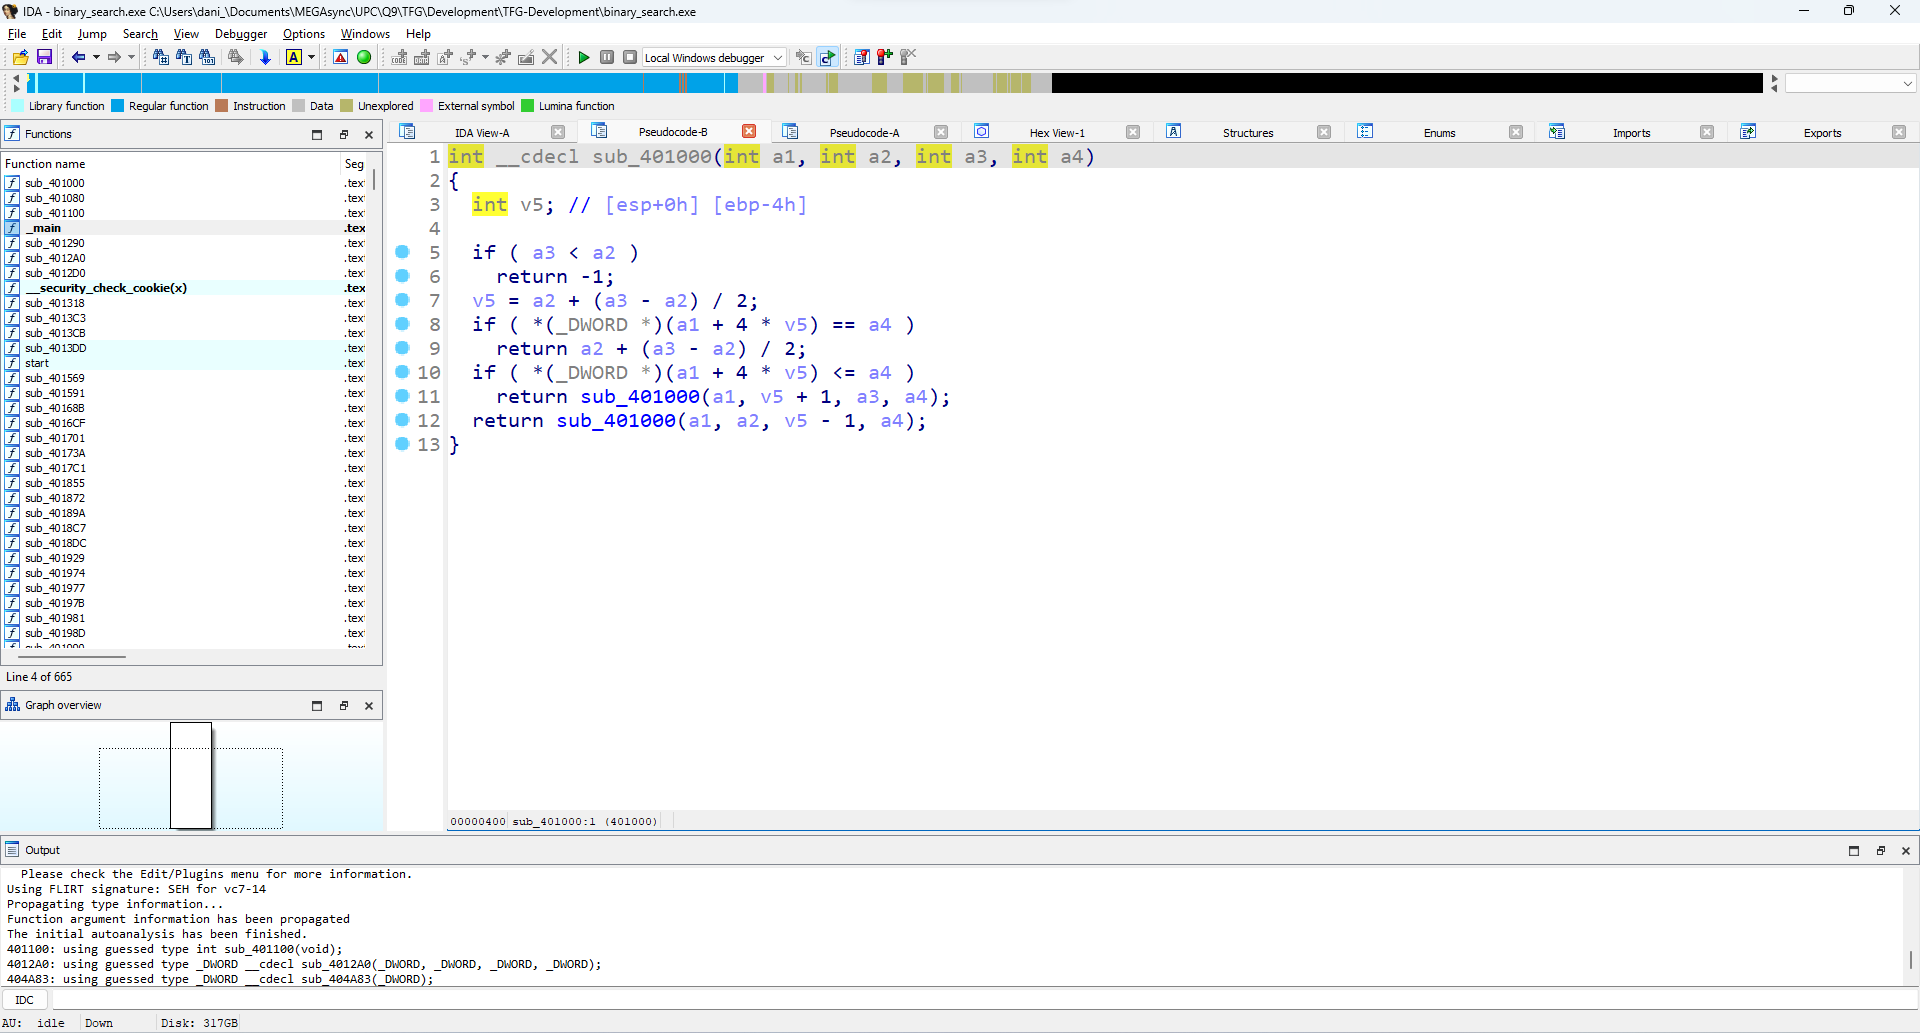
\includegraphics[width=15cm]{figuras/Capitulo_2/Cap_2_IDAPro_binaryseacrh1.png}
    \end{center}
    \caption[Captura de pantalla de IDA Free con el pseudocódigo generado para la funcion \textit{binaryseacrh1}]{Captura de pantalla de IDA Free con el pseudocódigo generado para la funcion \textit{binaryseacrh1} (Elaboración propia)}
    \label{fig:IDAPro_binaryseacrh1}
\end{figure}\

\begin{figure} [H]
    \begin{center}
      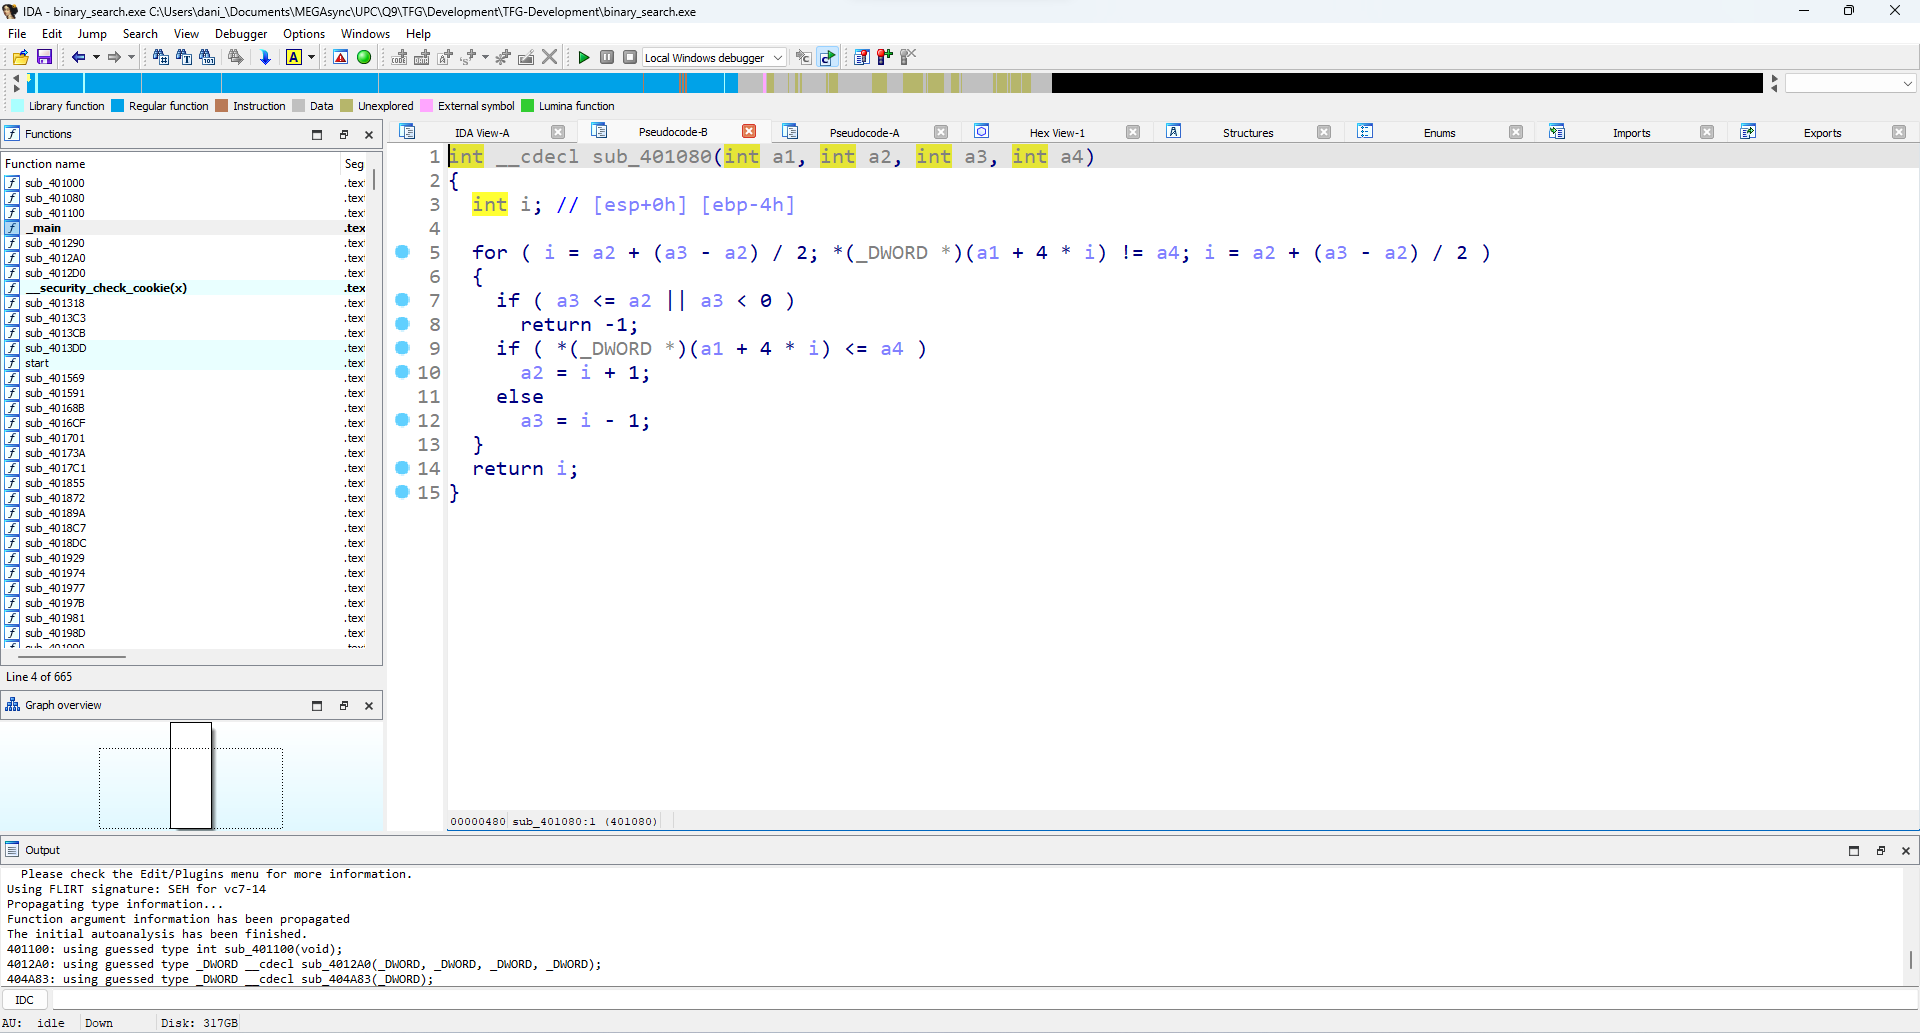
\includegraphics[width=15cm]{figuras/Capitulo_2/Cap_2_IDAPro_binaryseacrh2.png}
    \end{center}
    \caption[Captura de pantalla de IDA Free con el pseudocódigo generado para la funcion \textit{binaryseacrh2}]{Captura de pantalla de IDA Free con el pseudocódigo generado para la funcion \textit{binaryseacrh2} (Elaboración propia)}
    \label{fig:IDAPro_binaryseacrh2}
\end{figure}\

\section{Solucion tomada}
\label{sec:solucion}

% Corregido

Una vez visto en la sección \ref{sec:alternativas} las diferentes alternativas que hay en el mercado para poder aplicar ingeniería inversa sobre fichero ejecutable y observado que los
resultados obtenidos no son un código en C compilable y realista, quiero explicar cuál es la solución que en este proyecto se desarrollara.

El objetivo es a través de un ejecutable desamblado poder generar un código en C compilable y lo más fiel al original. Para ello queremos de asistirnos de la inteligencia artificial
de tal manera que si le damos un código desamblado esta nos pueda devolver un código en C. Más concretamente, queremos utilizar inteligencias artificiales basadas en redes neuronales
del estilo de ChatGPT\footnote{ChatGPT es una aplicación de chatbot de inteligencia artificial desarrollado en 2022 por OpenAI que se especializa en el diálogo} o modelos similares
como Llama\footnote{LLaMA (Large Language Model Meta AI) es un gran modelo de lenguaje (LLM) lanzado por Meta AI en febrero de 2023}.

Por lo tanto, lo que se pretende en esta solución es poder mejorar los resultados de decompiladores que hay en el mercado, asistiéndonos con inteligencia artificial, la cual ha demostrado
que a pesar de haber sido entrenadas para hacer una única tarea en concreto (los modelos anteriores por ejemplo, han sido entrenados exclusivamente para completar frases) son capaces de
realizar otro tipo de tareas a las cuales no han sido entrenadas y con resultados bastante buenos. Además, están pueden ser reentrenadas para mejorar los resultados.
